\setcounter{ProblemNumber}{1}
\ptwo{Plot the following points. \[(0,3), (-4,2), (3,-2), (-1,-2)\]
\begin{center}
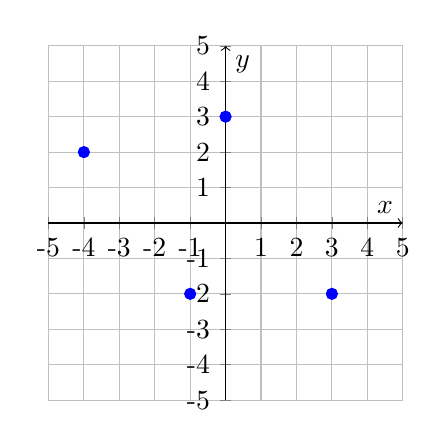
\begin{tikzpicture}
\begin{axis}[
    xmin=-5, xmax=5,
    ymin=-5, ymax=5,
    axis lines=center,
    axis on top=false,
    domain=0:1,
    x=0.45cm,
    y=0.45cm,
    xtick={-10,-9,...,10},
    xticklabels={-10,-9,...,10},
    ytick={-10,-9,...,10},
    yticklabels={-10,-9,...,10},
    axis lines=middle,
    axis line style={->},
    xlabel={$x$},
    ylabel={$y$},
    grid=major
    ]	
    \addplot [only marks,color=blue] table[row sep=crcr] {
	0 3\\
	3 -2\\
	-1 -2\\
	-4 2\\
	};
\end{axis}
\end{tikzpicture}
\end{center}
}
\ptwo{Plot the following points. \[(-3,1),(4,3),(2,-2),(1,-4)\]
\begin{center}
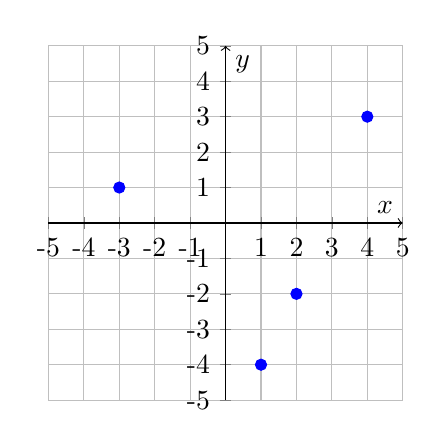
\begin{tikzpicture}
\begin{axis}[
    xmin=-5, xmax=5,
    ymin=-5, ymax=5,
    axis lines=center,
    axis on top=false,
    domain=0:1,
    x=0.45cm,
    y=0.45cm,
    xtick={-10,-9,...,10},
    xticklabels={-10,-9,...,10},
    ytick={-10,-9,...,10},
    yticklabels={-10,-9,...,10},
    axis lines=middle,
    axis line style={->},
    xlabel={$x$},
    ylabel={$y$},
    grid=major
    ]
    \addplot [only marks,color=blue] table[row sep=crcr] {
	4 3\\
	-3 1\\
	2 -2\\
	1 -4\\
	};
\end{axis}
\end{tikzpicture}
\end{center}
}

\ptwo{Graph the following line using the intercepts. \[2x+5y=10\]
\begin{center}
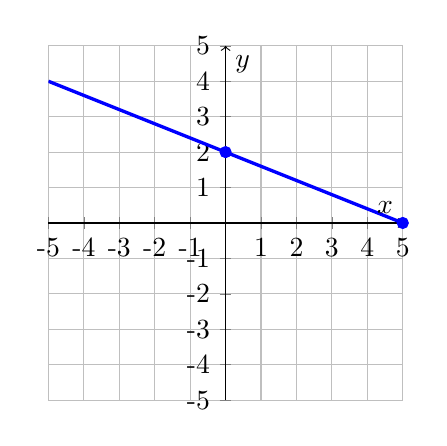
\begin{tikzpicture}
\begin{axis}[
    xmin=-5, xmax=5,
    ymin=-5, ymax=5,
    axis lines=center,
    axis on top=false,
    domain=0:1,
    x=0.45cm,
    y=0.45cm,
    xtick={-10,-9,...,10},
    xticklabels={-10,-9,...,10},
    ytick={-10,-9,...,10},
    yticklabels={-10,-9,...,10},
    axis lines=middle,
    axis line style={->},
    xlabel={$x$},
    ylabel={$y$},
    grid=major
    ]
    \addplot [only marks,color=blue] table[row sep=crcr] {
	0 2\\
	5 0\\
	};
	\addplot[samples=10,domain=-5:5,very thick, blue]{-2*x/5+2};
\end{axis}
\end{tikzpicture}
\end{center}}
\ptwo{Graph the following line using the intercepts. \[4x+3y=12\]
\begin{center}
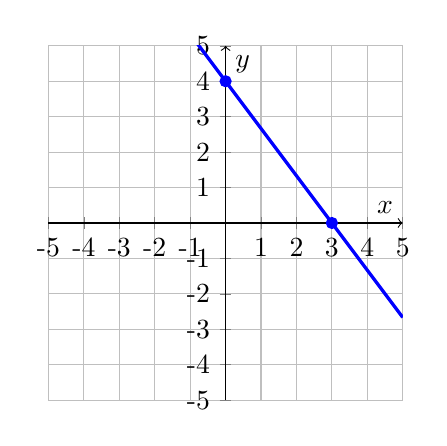
\begin{tikzpicture}
\begin{axis}[
    xmin=-5, xmax=5,
    ymin=-5, ymax=5,
    axis lines=center,
    axis on top=false,
    domain=0:1,
    x=0.45cm,
    y=0.45cm,
    xtick={-10,-9,...,10},
    xticklabels={-10,-9,...,10},
    ytick={-10,-9,...,10},
    yticklabels={-10,-9,...,10},
    axis lines=middle,
    axis line style={->},
    xlabel={$x$},
    ylabel={$y$},
    grid=major
    ]
    \addplot [only marks,color=blue] table[row sep=crcr] {
	0 4\\
	3 0\\
	};
	\addplot[samples=10,domain=-5:5,very thick, blue]{-4*x/3+4};
\end{axis}
\end{tikzpicture}
\end{center}}

\ptwo{Graph the following line using the intercepts. \[4x+4y=8\]
\begin{center}
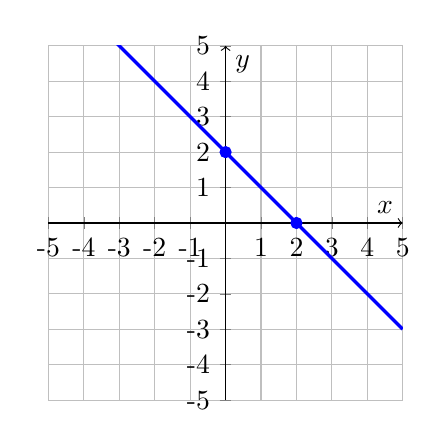
\begin{tikzpicture}
\begin{axis}[
    xmin=-5, xmax=5,
    ymin=-5, ymax=5,
    axis lines=center,
    axis on top=false,
    domain=0:1,
    x=0.45cm,
    y=0.45cm,
    xtick={-10,-9,...,10},
    xticklabels={-10,-9,...,10},
    ytick={-10,-9,...,10},
    yticklabels={-10,-9,...,10},
    axis lines=middle,
    axis line style={->},
    xlabel={$x$},
    ylabel={$y$},
    grid=major
    ]
    \addplot [only marks,color=blue] table[row sep=crcr] {
	0 2\\
	2 0\\
	};
	\addplot[samples=10,domain=-5:5,very thick, blue]{-x+2};
\end{axis}
\end{tikzpicture}
\end{center}}
\ptwo{Graph the following line using the intercepts. \[x+3y=3\]
\begin{center}
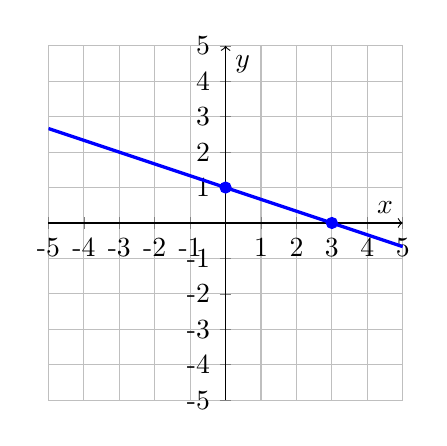
\begin{tikzpicture}
\begin{axis}[
    xmin=-5, xmax=5,
    ymin=-5, ymax=5,
    axis lines=center,
    axis on top=false,
    domain=0:1,
    x=0.45cm,
    y=0.45cm,
    xtick={-10,-9,...,10},
    xticklabels={-10,-9,...,10},
    ytick={-10,-9,...,10},
    yticklabels={-10,-9,...,10},
    axis lines=middle,
    axis line style={->},
    xlabel={$x$},
    ylabel={$y$},
    grid=major
    ]
    \addplot [only marks,color=blue] table[row sep=crcr] {
	0 1\\
	3 0\\
	};
	\addplot[samples=10,domain=-5:5,very thick, blue]{-x/3+1};
\end{axis}
\end{tikzpicture}
\end{center}}

\ptwo{Graph the following line using the slope and $y$-intercept. \[y=2x-3\]
\begin{center}
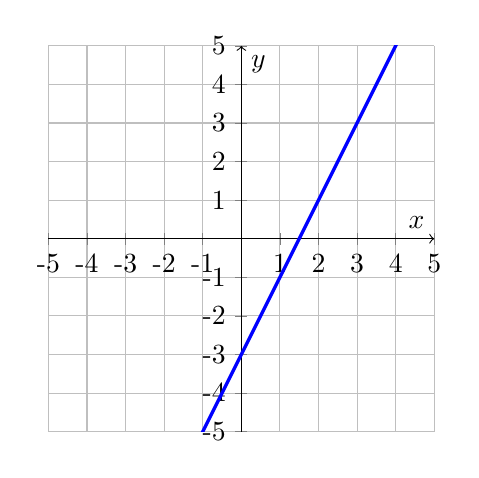
\begin{tikzpicture}
\begin{axis}[
    xmin=-5, xmax=5,
    ymin=-5, ymax=5,
    axis lines=center,
    axis on top=false,
    domain=0:1,
    x=0.49cm,
    y=0.49cm,
    xtick={-10,-9,...,10},
    xticklabels={-10,-9,...,10},
    ytick={-10,-9,...,10},
    yticklabels={-10,-9,...,10},
    axis lines=middle,
    axis line style={->},
    xlabel={$x$},
    ylabel={$y$},
    grid=major
    ]
    \addplot[samples=10,domain=-5:5,very thick, blue]{2*x-3};
\end{axis}
\end{tikzpicture}
\end{center}}
\ptwo{Graph the following line using the slope and $y$-intercept. \[y=-x+1\]
\begin{center}
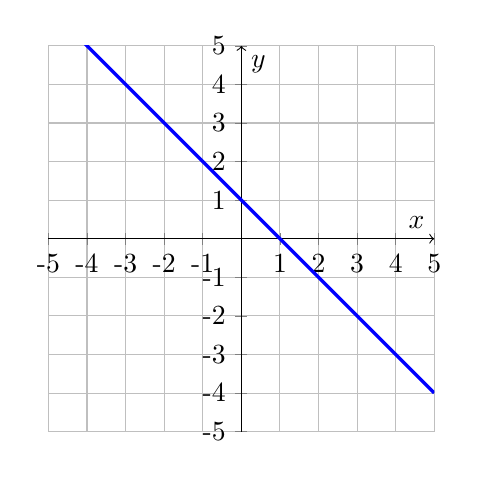
\begin{tikzpicture}
\begin{axis}[
    xmin=-5, xmax=5,
    ymin=-5, ymax=5,
    axis lines=center,
    axis on top=false,
    domain=0:1,
    x=0.49cm,
    y=0.49cm,
    xtick={-10,-9,...,10},
    xticklabels={-10,-9,...,10},
    ytick={-10,-9,...,10},
    yticklabels={-10,-9,...,10},
    axis lines=middle,
    axis line style={->},
    xlabel={$x$},
    ylabel={$y$},
    grid=major
    ]
    \addplot[samples=10,domain=-5:5,very thick, blue]{-x+1};
\end{axis}
\end{tikzpicture}
\end{center}}

\ptwo{Graph the following line using the slope and $y$-intercept. \[y=\dfrac{1}{2}x+4\]
\begin{center}
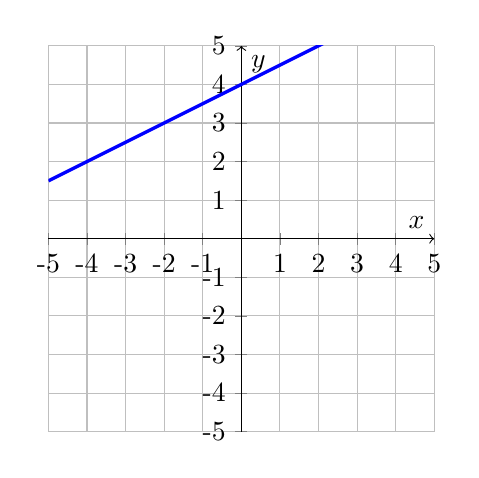
\begin{tikzpicture}
\begin{axis}[
    xmin=-5, xmax=5,
    ymin=-5, ymax=5,
    axis lines=center,
    axis on top=false,
    domain=0:1,
    x=0.49cm,
    y=0.49cm,
    xtick={-10,-9,...,10},
    xticklabels={-10,-9,...,10},
    ytick={-10,-9,...,10},
    yticklabels={-10,-9,...,10},
    axis lines=middle,
    axis line style={->},
    xlabel={$x$},
    ylabel={$y$},
    grid=major
    ]
    \addplot[samples=10,domain=-5:5,very thick, blue]{x/2+4};
\end{axis}
\end{tikzpicture}
\end{center}}
\ptwo{Graph the following line using the slope and $y$-intercept. \[x-3y=9\]
\begin{center}
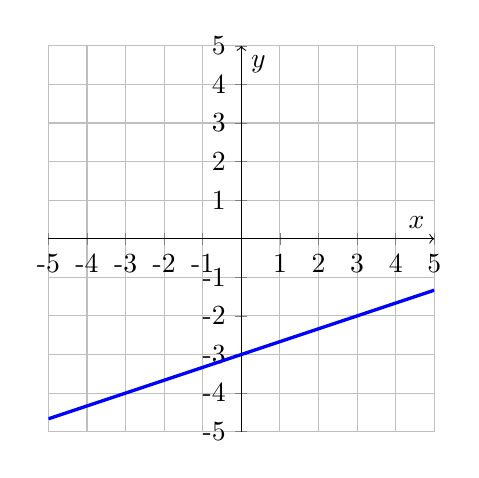
\begin{tikzpicture}
\begin{axis}[
    xmin=-5, xmax=5,
    ymin=-5, ymax=5,
    axis lines=center,
    axis on top=false,
    domain=0:1,
    x=0.49cm,
    y=0.49cm,
    xtick={-10,-9,...,10},
    xticklabels={-10,-9,...,10},
    ytick={-10,-9,...,10},
    yticklabels={-10,-9,...,10},
    axis lines=middle,
    axis line style={->},
    xlabel={$x$},
    ylabel={$y$},
    grid=major
    ]
    \addplot[samples=10,domain=-5:5,very thick, blue]{x/3-3};
\end{axis}
\end{tikzpicture}
\end{center}}

\ptwo{Graph the following line using any method. \[x+y=4\]
\begin{center}
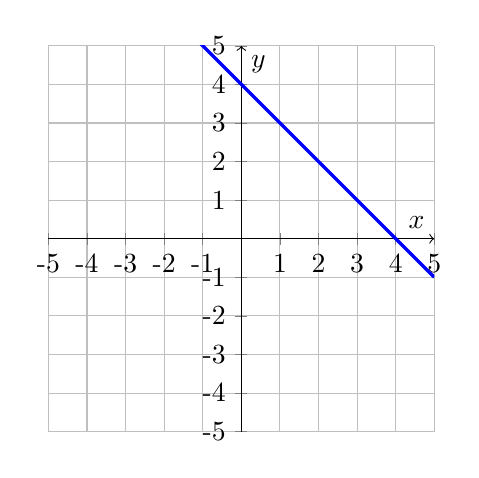
\begin{tikzpicture}
\begin{axis}[
    xmin=-5, xmax=5,
    ymin=-5, ymax=5,
    axis lines=center,
    axis on top=false,
    domain=0:1,
    x=0.49cm,
    y=0.49cm,
    xtick={-10,-9,...,10},
    xticklabels={-10,-9,...,10},
    ytick={-10,-9,...,10},
    yticklabels={-10,-9,...,10},
    axis lines=middle,
    axis line style={->},
    xlabel={$x$},
    ylabel={$y$},
    grid=major
    ]
    \addplot[samples=10,domain=-5:5,very thick, blue]{-x+4};
\end{axis}
\end{tikzpicture}
\end{center}}
\ptwo{Graph the following line using any method. \[-2x+3y=6\]
\begin{center}
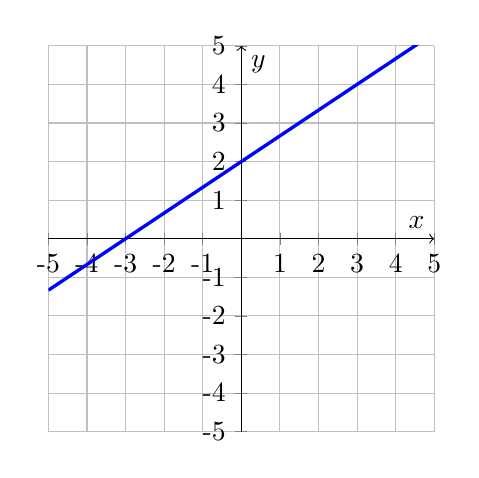
\begin{tikzpicture}
\begin{axis}[
    xmin=-5, xmax=5,
    ymin=-5, ymax=5,
    axis lines=center,
    axis on top=false,
    domain=0:1,
    x=0.49cm,
    y=0.49cm,
    xtick={-10,-9,...,10},
    xticklabels={-10,-9,...,10},
    ytick={-10,-9,...,10},
    yticklabels={-10,-9,...,10},
    axis lines=middle,
    axis line style={->},
    xlabel={$x$},
    ylabel={$y$},
    grid=major
    ]
    \addplot[samples=10,domain=-5:5,very thick, blue]{2*x/3+2};
\end{axis}
\end{tikzpicture}
\end{center}}

\ptwo{Graph the following line using any method. \[x=-3\]
\begin{center}
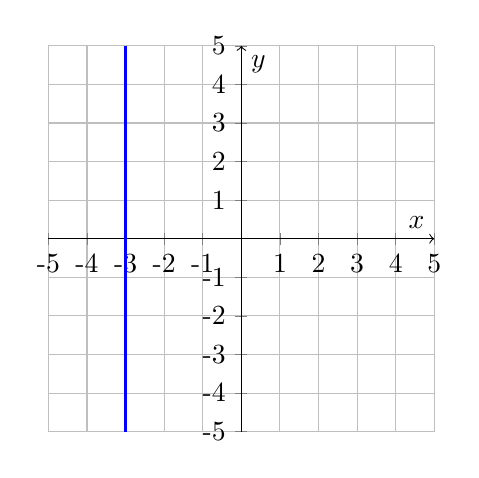
\begin{tikzpicture}
\begin{axis}[
    xmin=-5, xmax=5,
    ymin=-5, ymax=5,
    axis lines=center,
    axis on top=false,
    domain=0:1,
    x=0.49cm,
    y=0.49cm,
    xtick={-10,-9,...,10},
    xticklabels={-10,-9,...,10},
    ytick={-10,-9,...,10},
    yticklabels={-10,-9,...,10},
    axis lines=middle,
    axis line style={->},
    xlabel={$x$},
    ylabel={$y$},
    grid=major
    ]
    \addplot [blue,very thick] coordinates{(-3,-5)(-3,5)};
\end{axis}
\end{tikzpicture}
\end{center}}
\ptwo{Graph the following line using any method. \[2y+x=4\]
\begin{center}
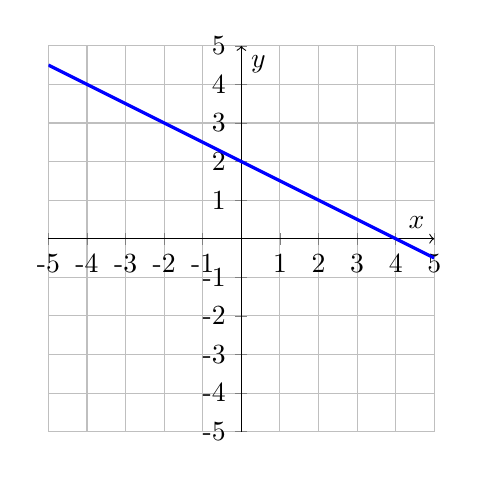
\begin{tikzpicture}
\begin{axis}[
    xmin=-5, xmax=5,
    ymin=-5, ymax=5,
    axis lines=center,
    axis on top=false,
    domain=0:1,
    x=0.49cm,
    y=0.49cm,
    xtick={-10,-9,...,10},
    xticklabels={-10,-9,...,10},
    ytick={-10,-9,...,10},
    yticklabels={-10,-9,...,10},
    axis lines=middle,
    axis line style={->},
    xlabel={$x$},
    ylabel={$y$},
    grid=major
    ]
    \addplot[samples=10,domain=-5:5,very thick, blue]{-x/2+2};
\end{axis}
\end{tikzpicture}
\end{center}}

\ptwo{Graph the following line using any method. \[y=2\]
\begin{center}
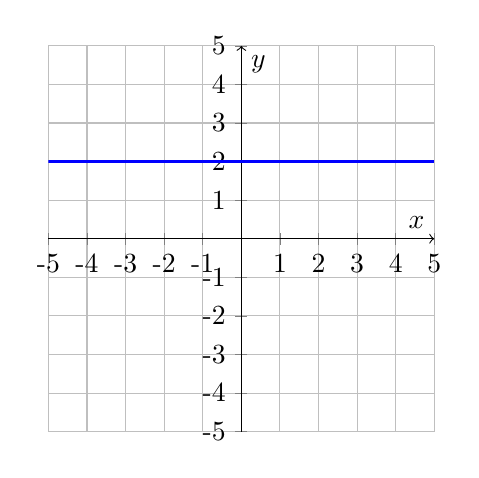
\begin{tikzpicture}
\begin{axis}[
    xmin=-5, xmax=5,
    ymin=-5, ymax=5,
    axis lines=center,
    axis on top=false,
    domain=0:1,
    x=0.49cm,
    y=0.49cm,
    xtick={-10,-9,...,10},
    xticklabels={-10,-9,...,10},
    ytick={-10,-9,...,10},
    yticklabels={-10,-9,...,10},
    axis lines=middle,
    axis line style={->},
    xlabel={$x$},
    ylabel={$y$},
    grid=major
    ]
    \addplot [blue,very thick] coordinates{(-5,2)(5,2)};
\end{axis}
\end{tikzpicture}
\end{center}}
\ptwo{Graph the following line using any method. \[3x+2y=4\]
\begin{center}
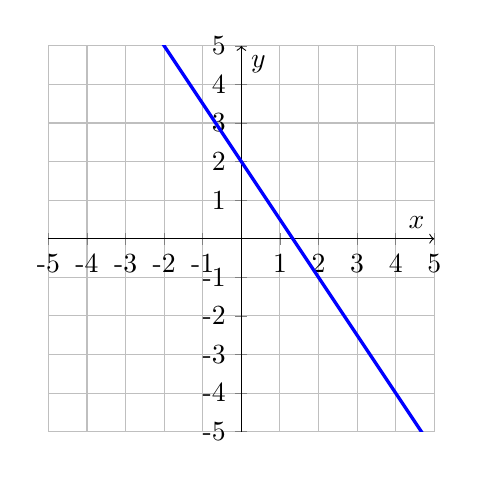
\begin{tikzpicture}
\begin{axis}[
    xmin=-5, xmax=5,
    ymin=-5, ymax=5,
    axis lines=center,
    axis on top=false,
    domain=0:1,
    x=0.49cm,
    y=0.49cm,
    xtick={-10,-9,...,10},
    xticklabels={-10,-9,...,10},
    ytick={-10,-9,...,10},
    yticklabels={-10,-9,...,10},
    axis lines=middle,
    axis line style={->},
    xlabel={$x$},
    ylabel={$y$},
    grid=major
    ]
    \addplot[samples=10,domain=-5:5,very thick, blue]{-3*x/2+2};
\end{axis}
\end{tikzpicture}
\end{center}}

\ptwo{Graph the following line using any method. \[-5x-4y=12\]
\begin{center}
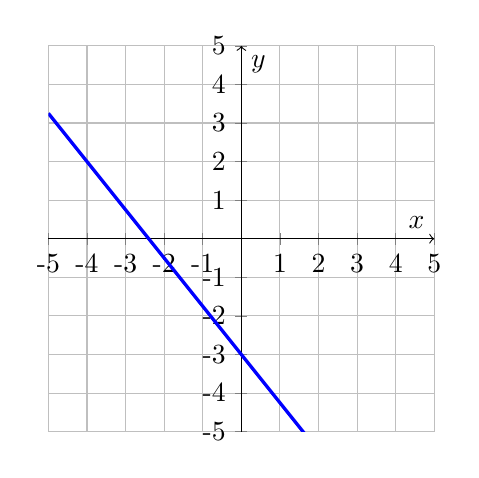
\begin{tikzpicture}
\begin{axis}[
    xmin=-5, xmax=5,
    ymin=-5, ymax=5,
    axis lines=center,
    axis on top=false,
    domain=0:1,
    x=0.49cm,
    y=0.49cm,
    xtick={-10,-9,...,10},
    xticklabels={-10,-9,...,10},
    ytick={-10,-9,...,10},
    yticklabels={-10,-9,...,10},
    axis lines=middle,
    axis line style={->},
    xlabel={$x$},
    ylabel={$y$},
    grid=major
    ]
    \addplot[samples=10,domain=-5:5,very thick, blue]{-5*x/4-3};
\end{axis}
\end{tikzpicture}
\end{center}}
\ptwo{Graph the following line using any method. \[y=-3x+5\]
\begin{center}
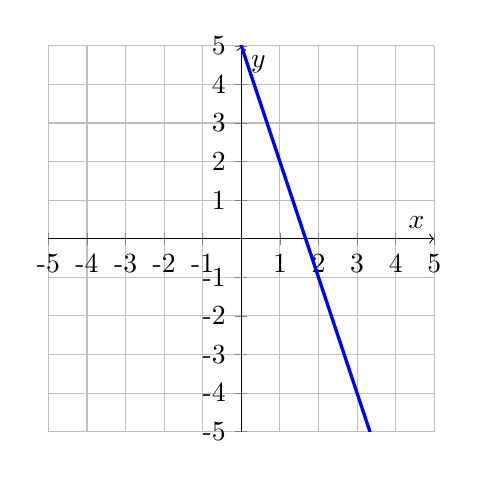
\begin{tikzpicture}
\begin{axis}[
    xmin=-5, xmax=5,
    ymin=-5, ymax=5,
    axis lines=center,
    axis on top=false,
    domain=0:1,
    x=0.49cm,
    y=0.49cm,
    xtick={-10,-9,...,10},
    xticklabels={-10,-9,...,10},
    ytick={-10,-9,...,10},
    yticklabels={-10,-9,...,10},
    axis lines=middle,
    axis line style={->},
    xlabel={$x$},
    ylabel={$y$},
    grid=major
    ]
    \addplot[samples=10,domain=-5:5,very thick, blue]{-3*x+5};
\end{axis}
\end{tikzpicture}
\end{center}}